\documentclass[tikz,border=2pt]{standalone}
\usepackage{tikz}
\usetikzlibrary{positioning}
\begin{document}
	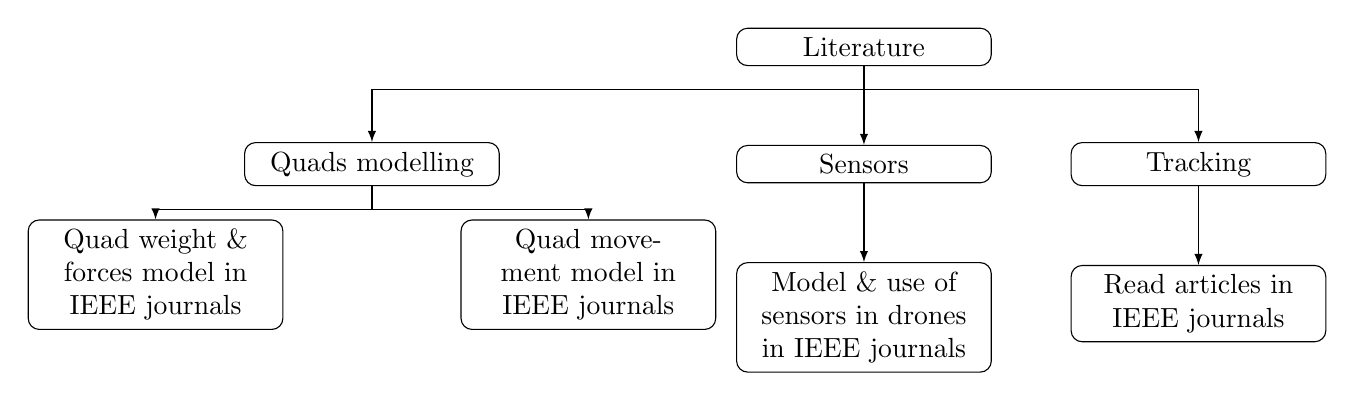
\begin{tikzpicture}[
	main/.style={rectangle, rounded corners, text centered, text width=3cm, draw=black},
	aux/.style={}
	]	

						
		\node (lit) [main] {Literature};
			\node (sensorslit) [main, below=of lit] {Sensors};
				\node (sensorsjour) [main, below=of sensorslit] {Model \& use of sensors in drones in IEEE journals};
			\node (modlit) [main, left=3cm of sensorslit] {Quads modelling};
				\node (aux3) [aux, below=of modlit] {};
				\node(weighandforces)[main, left=of aux3] {Quad weight \& forces model in IEEE journals};
				\node(movement)[main, right=of aux3] {Quad movement model in IEEE journals};
			\node (trackinglit) [main, right=of sensorslit] {Tracking};
				\node (trackjour) [main, below=of trackinglit] {Read articles in IEEE journals};
		

	
	\draw [-latex] (lit.south)--++(0,-.3)-| (modlit.north);
	\draw [-latex] (lit.south)--++(0,-.3)-| (sensorslit.north);
	\draw [-latex] (lit.south)--++(0,-.3)-| (trackinglit.north);
	
		
	\draw [-latex] (modlit.south)--++(0,-.3)-| (weighandforces.north);	
	\draw [-latex] (modlit.south)--++(0,-.3)-| (movement.north);
	\draw [-latex] (sensorslit.south)--++(0,-.3)-| (sensorsjour.north);	
	\draw [-latex] (trackinglit.south)--++(0,-.3)-| (trackjour.north);	

	
	\end{tikzpicture}
\end{document}